\section{Theoretical Analysis}
\label{sec:propwork-casod-theory}

\subsection{Qualitative Justification}

%{\color{blue}To mathematically support this in \sys, note that the SA attention matrix is computed from the concatenated view features $A_{SA} \in \mathbb{R}^{3T \times 3T}$, while the CVCA attention matrices are computed from two view features $A_{CVCA,v1 \rightarrow v2} \in \mathbb{R}^{T \times T}$. This implies that the denominator of the softmax in $A_{SA}$ is greater than the denominator of the softmax in each $A_{CVCA,v1 \rightarrow v2}$, $\sum_{j=1}^{3T} e^{a_{SA,j}} > \sum_{j=1}^{T} e^{a_{CVCA,j}}$ where $a$ is the pre-softmax attention value. Furthermore, CVCA is the sum of both view attention matrices $A_{CVCA} = A_{CVCA,v1 \rightarrow v2} + A_{CVCA,v2 \rightarrow v1}$. Following from these, SA \textbf{reduces} the magnitude of both patch activations while CVCA \textbf{additively reinforces} them. See Appendix Sec. E.2 for further analysis details.} %\sys performs significantly better. %While MaxPooling is sometimes superior for simpler far-OOD datasets, the feature details learned via bidirectional cross-view attention are crucial for near-OOD datasets. %Max-pooling is unable to learn these discriminative features and is weak at detecting near-OOD samples.
%{\color{purple}
The performance of CASOD fundamentally depends on the CVCA operation in the proposed fusion architecture. The significance of this operation is demonstrated via a comparison between CVCA attention computations and the standard self-attention (SA) computations in Transformer models \cite{vaswani2017attention} and throughout modern deep learning literature \cite{vaswani2017attention,dosovitskiy2020image,khan2023survey}. The theoretical analysis presented in this section begins with a high-level qualitative justification which can be read as a mathematical introduction to the theory to follow. To assist, please refer to \ref{fig:casod_model_arch} for an illustration of the CVCA architecture. The multi-view SA architecture considered here uses a concatenated view feature as input to an SA block (see \ref{fig:bkgd-attn_example} for an illustration). Thus, the comparison is between CVCA and SA as a fusion mechanism for discriminative feature learning and subsequent OOD detection. The motivating question is if CVCA offers improvements over SA.

\begin{figure*}
	\centering
	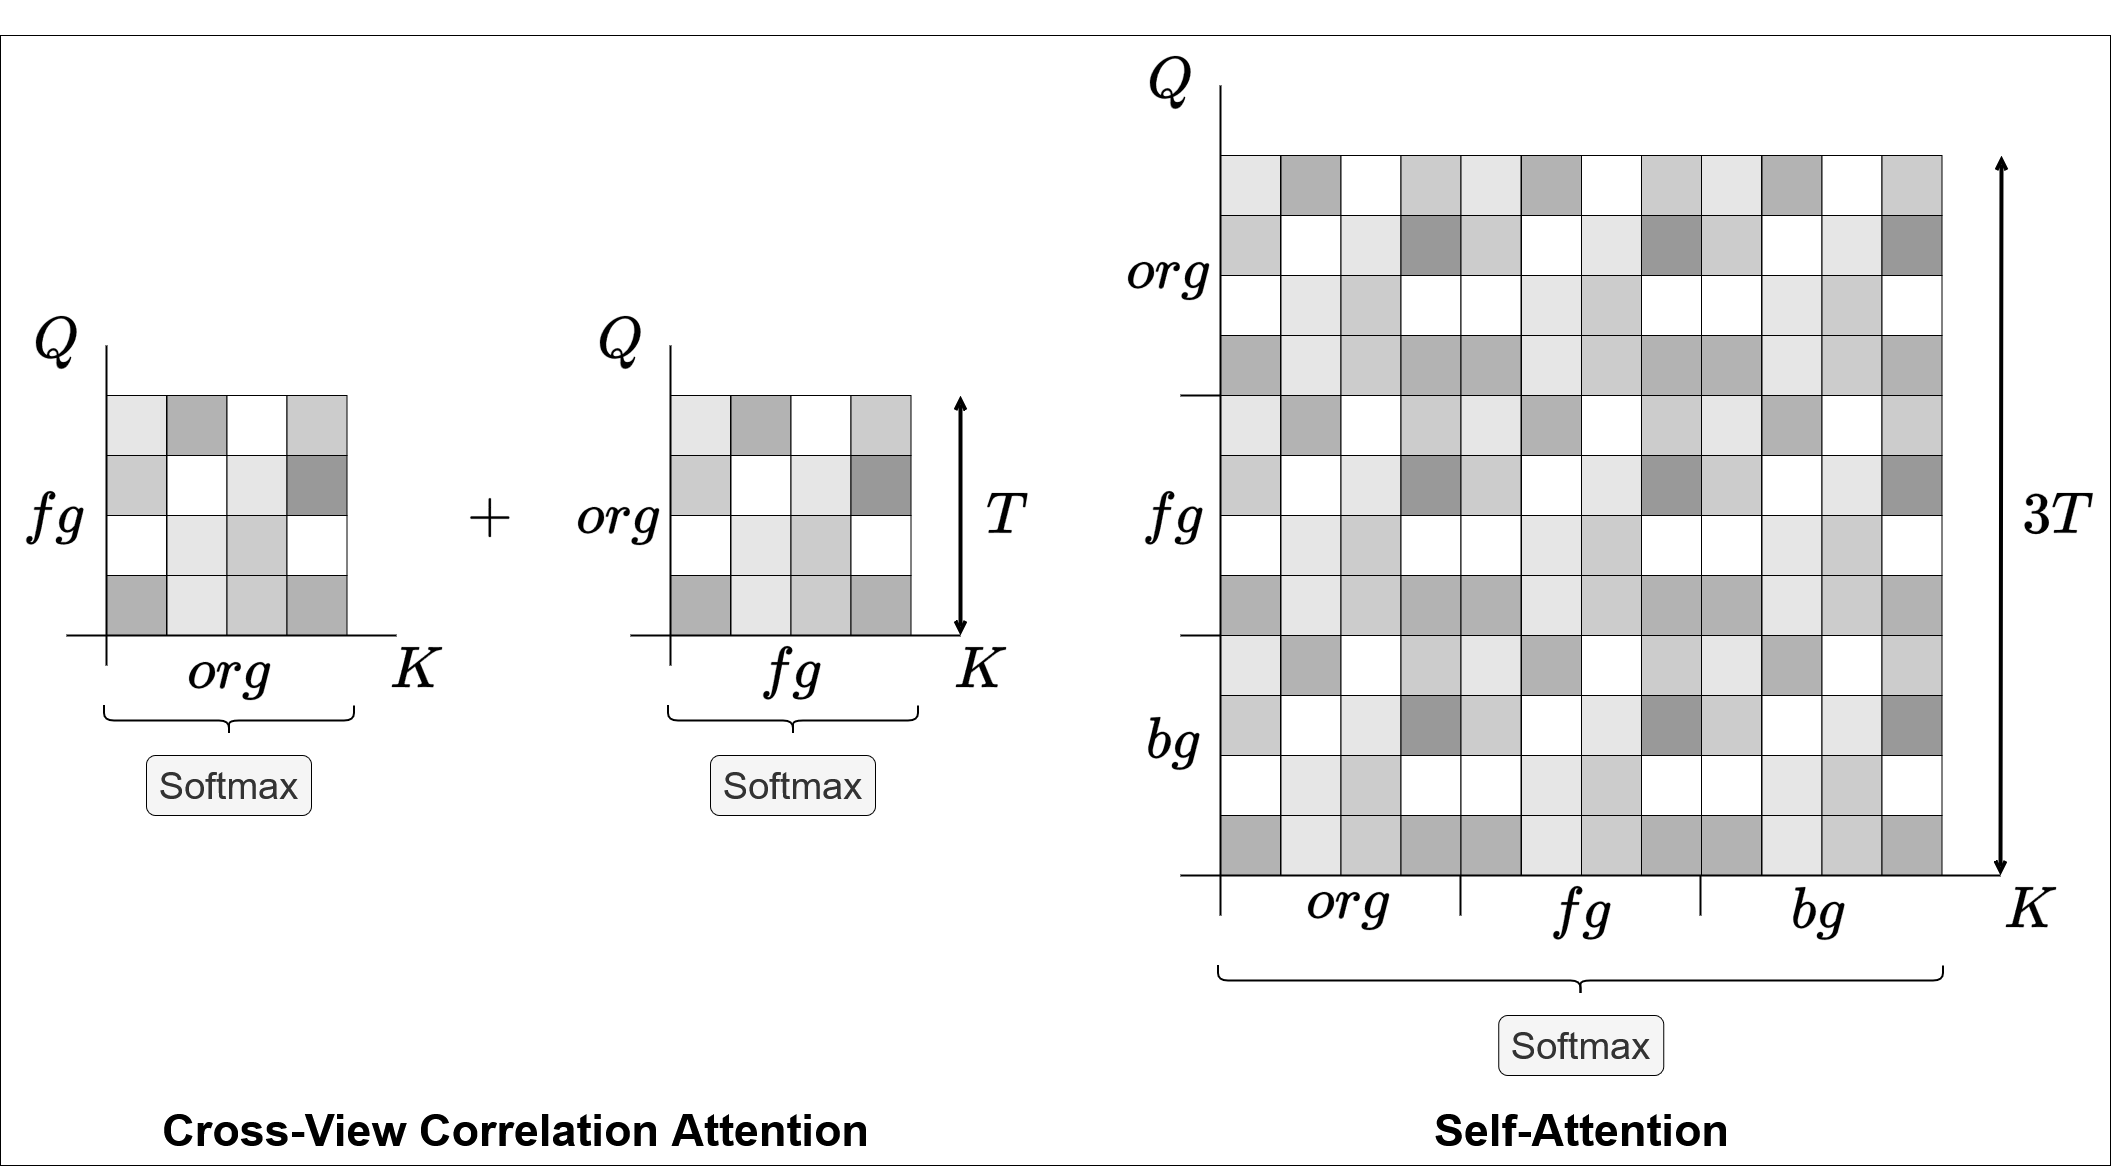
\includegraphics[width=1.\linewidth]{figures/matrix_attention_describe}
	\caption{The attention matrices in CVCA and SA are completely different, with CVCA allowing for \textbf{higher attention values} across features. The addition of cross-view attention matrices and smaller token dimensions in CVCA ensure greater emphasis of view features.
	}
	\label{fig:theory_matrix_ref}
\end{figure*}

SA attention matrices $A_{SA} \in \mathbb{R}^{3T \times 3T}$ are computed from the \emph{concatenated} view features (see \ref{fig:theory_matrix_ref}). CVCA attention matrices $A_{CVCA,v1 \rightarrow v2} \in \mathbb{R}^{T \times T}$ are computed from two view features (see \ref{fig:theory_matrix_ref}). Given identical input features $\tilde{z}$ and weight matrices $W_Q, W_K$, the higher dimensionality of SA attention matrices guarantees that the denominator of the softmax in $A_{SA}$ is greater than the denominator of the softmax in each $A_{CVCA,v1 \rightarrow v2}$, i.e. $\sum_{j=1}^{3T} e^{a_{SA,j}} > \sum_{j=1}^{T} e^{a_{CVCA,j}}$ where $a$ is the pre-softmax attention value. Furthermore, CVCA is the sum of both view attention matrices $A_{CVCA} = A_{CVCA,v1 \rightarrow v2} + A_{CVCA,v2 \rightarrow v1}$. In this setting, SA \textbf{reduces} the magnitude of patch activations while CVCA \textbf{additively reinforces} them.

However, in practice, it is not guaranteed that the input features $\tilde{z}$ nor the weight matrices $W_Q, W_K$ are the same in both SA and CVCA architectures. A more principled analysis is beneficial in isolating the conditions for CVCA to improve upon SA.
%}

%\subsection{Assumptions and Prerequisites}
%
%{\color{purple}
%
%}

%\subsection{Guarantees}
\subsection{Theoretical Findings}

%{\color{blue}
%(\textbf{NEW ATTEMPT} %general direction idea: if we can show org, fg, bg features are approximately the same under each paradigm, then this is guaranteed)
%Consider a particular high-activation patch in the CVCA attention matrix $p^* \in A_{CVCA,i}$ at index $j$. Assume the patch is exclusively from only one of the view attention matrices $p^* = \text{softmax}(z_{v1} W_{Q,v1} W_{K,v2}^{\intercal} z_{v2}^{\intercal})_{i,j} + 0$. We also distinguish the patch probabilities $p$ and the patch values before softmax as $a$.
%
%We analyze the conditions for self-attention to similarly identify and emphasize this critical high-attention patch. That is, $p^*_{SA} \geq p^*_{CVCA}$. We rewrite this expression as follows:
%\begin{equation}
%    \frac{e^{a^*_{SA}}}{\sum_{3T} e^{a_{SA}}} \geq \frac{e^{a^*_{CVCA}}}{\sum_{T} e^{a_{CVCA}}}
%\end{equation}
%\begin{equation}
%    e^{a^*_{SA}} \geq e^{a^*_{CVCA}} \frac{\sum_{3T} e^{a_{SA}}}{\sum_{T} e^{a_{CVCA}}}
%\end{equation}
%\begin{equation}
%    a^*_{SA} \geq a^*_{CVCA} + \ln{(\sum_{3T} e^{a_{SA}})} - \ln{(\sum_{T} e^{a_{CVCA}})}
%\end{equation}
%\begin{align}
%    a^*_{SA} \geq\ & a^*_{CVCA} + \ln{(e^{a^*_{SA}})} + \ln{(1 + \sum_{3T-1} \frac{e^{a_{SA}}}{e^{a^*_{SA}}})} \\
%    & - \ln{(e^{a^*_{CVCA}})} - \ln{(1 + \sum_{T-1} \frac{e^{a_{CVCA}}}{e^{a^*_{CVCA}}})}
%\end{align}
%\begin{equation}
%    1 + \sum_{T-1} \frac{e^{a_{CVCA}}}{e^{a^*_{CVCA}}} \geq 1 + \sum_{3T-1} \frac{e^{a_{SA}}}{e^{a^*_{SA}}}
%\end{equation}
%\begin{equation}
%    \frac{\sum_{T-1} e^{a_{CVCA}}}{\sum_{3T-1} e^{a_{SA}}} \geq e^{a^*_{CVCA} - a^*_{SA}}
%\end{equation}
%
%We show that this condition is not satisfied in the general case with high probability. We make two assumptions following from existing theoretical work:
%\begin{itemize}
%    \item \textbf{Assumption 1} The intermediate features $z$ in both SA and CVCA are bounded [A1].
%    \item \textbf{Assumption 2} The weight matrices $W_Q$, $W_K$, and $W_V$ in both SA and CVCA are bounded [A2,A3].
%\end{itemize}
%
%% from before:
%% https://proceedings.mlr.press/v119/xiong20b/xiong20b.pdf
%% https://arxiv.org/pdf/2305.03210
%% new potential:
%% https://arxiv.org/pdf/1511.07543 (not guaranteed same)
%% https://dl.acm.org/doi/pdf/10.1145/3728458 (not guaranteed same)
%% 
%
%%Assumption 1 is given through the concentration properties of LayerNorm operations. Assumption 2 is fundamental to efficient attention computation in practice. These assumptions immediately give that the patch values $a_{SA}$ and $a_{CVCA}$ are also bounded. {\color{red}TODO: what to do from here? are any of these options feasible?
%%\begin{enumerate}
%%    \item claim that $a^*_{CVCA} \approx a^*_{SA}$ from optimizing the same objective, then try and show the left-hand side denominator will almost always be larger than the numerator
%%    \item claim that $z$ are similar in SA and CVCA due to optimization of the same objective, claim that all Q, K project to similar attention matrices for SA and CVCA due to optimization of the same objective
%%    \item 
%%\end{enumerate}
%%}
%}
%{\color{purple}

\subsubsection{Preliminary Information}
Self-attention (SA) and cross-attention (CA) are reiterated here (see Chapter \ref{diss_bkgd} for further details). Note that notations here generally follow those presented in Chapter \ref{diss_bkgd} for Attention mechanisms but more specifically follow those in the previous section for CVCA (Section \ref{sec:propwork-casod-method}). The exception is that inputs (i.e. features) for the rest of this section are represented as $x$ instead of $\tilde{z}$ for generality. In SA,
an input $x$ is projected into matrices $Q$, $K$, and $V$ using respective parameters $W_Q \in \mathbb{R}^{d \times d_k}$, $W_K \in \mathbb{R}^{d \times d_k}$, $W_V \in \mathbb{R}^{d \times d_v}$
\begin{equation}
\begin{aligned}
    Q & = x W_Q \\
    K & = x W_K \\
    V & = x W_V. \\
\end{aligned}
\end{equation}
The attention $A$ is calculated from $Q$, $K$, and $V$, intermediary attention values $\alpha$, and the softmax function
\begin{equation}
\begin{aligned}
    \alpha(Q,K,d_k) & = \text{softmax} (\frac{Q K^{\mathsf{T}}}{\sqrt{d_k}}) \\
    A(\alpha,V) & = \alpha V.
\end{aligned}
\end{equation}
The softmax function is defined as follows
\begin{equation}
\begin{aligned}
    o(x)_i = \frac{e^{x_i}}{\sum_{j=1}^{K} e^{x_j}}, \\
\end{aligned}
\end{equation}
for some vector $x \in \mathbb{R}^K$ and resulting in vector $o(x) \in (0,1)^K$. Intermediary attention values $\alpha$ and attention values $A$ can be further delineated by patch. That is, for patch indices $i,j$
\begin{equation}
\begin{aligned}
    \alpha_{ij} & = \text{softmax} (\frac{Q_i K_j^{\mathsf{T}}}{\sqrt{d_k}}), \\
\end{aligned}
\end{equation}
and similar for any $A_{ij}$.
CA takes as input two inputs $x_1$ and $x_2$. $Q$, $K$, and $V$ are computed
\begin{equation}
\begin{aligned}
    Q & = x_1 W_Q \\
    K & = x_2 W_K \\
    V & = x_2 W_V, \\
\end{aligned}
\end{equation}
before attention is calculated. Note that parameters in CA are labeled according to their respective origin input, e.g. $Q_1$, $K_2$
\begin{equation}
\begin{aligned}
    \alpha(Q_1,K_2,d_k) & = \text{softmax} (\frac{Q_1 K_2^{\mathsf{T}}}{\sqrt{d_k}}) \\
    A(\alpha,V_2) & = \alpha V_2.
\end{aligned}
\end{equation}

Cross-view correlation attention (CVCA), proposed in the previous section (see Section \ref{sec:propwork-casod-method}), is inspired by CA and considers inputs from two views $x_{v1}, x_{v2}$. Attention is computed using view-associated preliminary attention values $\alpha_{12}, \alpha_{21}$ as follows
\begin{equation}
\begin{aligned}
    Q_{1,v1} & = x_{v1} W_{Q,1} \\
    K_{1,v2} & = x_{v2} W_{K,1} \\
    Q_{2,v2} & = x_{v2} W_{Q,2} \\
    Q_{2,v1} & = x_{v1} W_{K,2} \\
    \alpha_{12} & = \text{softmax} (\frac{Q_{1,v1} K_{1,v2}^{\mathsf{T}}}{\sqrt{d_{k_{v1}}}}) \\
    \alpha_{21} & = \text{softmax} (\frac{Q_{2,v2} K_{2,v1}^{\mathsf{T}}}{\sqrt{d_{k_{v2}}}}) \\
    \alpha & = \alpha_{12} + \alpha_{21}. \\
\end{aligned}
\end{equation}
Each preliminary attention value is computed with a corresponding $Q,K$, with $\alpha_{12}$ using $Q_1,K_1$ and $\alpha_{21}$ using $Q_2,K_2$.
%Any preliminary attention value $\alpha$ can be further delineated as the raw attention values $a$ prior to application of the softmax function, that is
%\begin{equation}
%\begin{aligned}
%    a_{ij} & = (\frac{Q_i K_j^{\mathsf{T}}}{\sqrt{d_k}}) \\
%    \alpha_{ij} & = \text{softmax} (a_{ij}). \\
%\end{aligned}
%\end{equation}
Henceforth in this section, the preliminary attention values $\alpha$ are referred to equivalently as the ``attention values'' or generally as ``attention'' in SA and CVCA.

For SA, the input $x$ in multi-view systems is a combination of all views, that is the original view $x_{org}$, the foreground view $x_{fg}$, and the background view $x_{bg}$. Specifically, $x$ in SA is a concatenation of all three view features
\begin{equation}
\begin{aligned}
    x = [x_{org} ; x_{fg} ; x_{bg}], \\
\end{aligned}
\end{equation}
with $x \in \mathbb{R}^{3T \times d}$, as each view feature $x_v \in \mathbb{R}^{T \times d}$ for $v \in \{org, fg, bg\}$. Each input for CVCA is exactly one of $x_{org}, x_{fg}, x_{bg}$.

\subsubsection{Main Findings}
Consider a discriminative high-activation patch $\alpha^*_{CVCA}$ in a CVCA attention matrix $\alpha^*_{CVCA} = \alpha_{CVCA,i^*j^*}$ for row $i^*$ at index $j^*$. Here, only one of the preliminary attention matrices is considered for comparison, i.e. only $\alpha_{12}$. The relationship between SA and CVCA for this discriminative high-activation patch can be expressed as
\begin{equation}
\begin{aligned}
    \alpha^*_{SA} \? \alpha^*_{CVCA}, \\
\end{aligned}
\label{peqn:1}
\end{equation}
where the $\?$ operator delineates an unknown relationship between the two operands. The goal is to identify the relationship between the two attention values and replacing the $\?$ operator with an informative, formal inequality. In CVCA, $\alpha_{12}$ must include $x_{org}$ as one of the inputs ($x_1$ for the rest of the analysis) and $x_2 = x_{fg}$ is considered as the other input without loss of generality. The expansion of \ref{peqn:1} follows by taking the softmax of both sides
\begin{equation}
\begin{aligned}
    %\alpha^*_{SA}  \alpha^*{CVCA}. \\
    \frac{e^{\alpha^*_{SA}}}{\sum_{k=1}^{3T} e^{\alpha_{SA,k}}} \? \frac{e^{\alpha^*_{CVCA}}}{\sum_{k=1}^{T} e^{\alpha_{CVCA,k}}}. \\
\end{aligned}
\label{peqn:2}
\end{equation}
The expression \ref{peqn:2} can be rearranged as such
\begin{align}
    %\alpha^*_{SA}  \alpha^*{CVCA}. \\
    e^{\alpha^*_{SA}} & \? e^{\alpha^*_{CVCA}} \frac{\sum_{k=1}^{3T} e^{\alpha_{SA,k}}}{\sum_{k=1}^{T} e^{\alpha_{CVCA,k}}} \nonumber \\
    \alpha^*_{SA} & \? \ln (e^{\alpha^*_{CVCA}}) + \ln (\sum_{k=1}^{3T} e^{\alpha_{SA,k}}) - \ln (\sum_{k=1}^{T} e^{\alpha_{CVCA,k}}) \nonumber \\
    \alpha^*_{SA} & \? \alpha^*_{CVCA} + \ln (e^{\alpha^*_{SA}}) + \ln (1 + \sum_{k=1}^{3T-1} \frac{e^{\alpha_{SA,k}}}{e^{\alpha^*_{SA}}}) - \ln (e^{\alpha^*_{CVCA}}) - \ln (1 + \sum_{k=1}^{T-1} \frac{e^{\alpha_{CVCA,k}}}{e^{\alpha^*_{CVCA}}}). \label{peqn:3}
\end{align}
The isolation of the $\alpha^*_{SA}, \alpha^*_{CVCA}$ terms from the summations follows from the analysis of the summation, here shown for the SA term but identically applicable to the CVCA term
\begin{equation}
\begin{aligned}
    \ln (\sum_{k=1}^{3T} e^{\alpha_{SA,k}}) & = e^{\alpha^*_{SA}} + e^{\alpha_{SA,1}} + e^{\alpha_{SA,2}} + \dots \\
    & = \ln (e^{\alpha^*_{SA}} (1 + \frac{e^{\alpha_{SA,1}}}{e^{\alpha^*_{SA}}} + \frac{e^{\alpha_{SA,2}}}{e^{\alpha^*_{SA}}} + \dots)) \\
    & = \ln (e^{\alpha^*_{SA}}) + \ln (1 + \sum_{k=1}^{3T-1} \frac{e^{\alpha_{SA,k}}}{e^{\alpha^*_{SA}}}). \\
\end{aligned}
\end{equation}
It is assumed that the discriminative high-activation patches $\alpha^*$ represent discriminative features learned by the model and are thus nearly identical in both SA and CVCA.
\begin{assumption}
    $\alpha^*_{SA} = \alpha^*_{CVCA} + E^*,$ \\
    $\cancelto{\simeq 0}{E^*}$ \\
    %$\cancelto{\approx 0}{A}$
    for some error $E^*$.
\label{pass:1}
\end{assumption}
%\begin{align}
%    %\alpha^*_{SA}  \alpha^*{CVCA}. \\
%    e^{\alpha^*_{SA}} & \? e^{\alpha^*_{CVCA}} \frac{\sum_{k=1}^{3T} e^{\alpha_{SA,k}}}{\sum_{k=1}^{T} e^{\alpha_{CVCA,k}}} \\
%    \alpha^*_{SA} & \? \ln (e^{\alpha^*_{CVCA}}) + \ln (\sum_{k=1}^{3T} e^{\alpha_{SA,k}}) - \ln (\sum_{k=1}^{T} e^{\alpha_{CVCA,k}}) \\
%    \alpha^*_{SA} & \? \alpha^*_{CVCA} + \ln (e^{\alpha^*_{SA}}) + \ln (1 + \sum_{k=1}^{3T-1} \frac{e^{\alpha_{SA,k}}}{e^{\alpha^*_{SA}}}) - \ln (e^{\alpha^*_{CVCA}}) - \ln (1 + \sum_{k=1}^{T-1} \frac{e^{\alpha_{CVCA,k}}}{e^{\alpha^*_{CVCA}}}). \\
%\end{align}
\ref{peqn:3} can be further simplified as follows
\begin{align}
    0 & \? \ln (1 + \sum_{k=1}^{3T-1} \frac{e^{\alpha_{SA,k}}}{e^{\alpha^*_{SA}}}) - \ln (1 + \sum_{k=1}^{T-1} \frac{e^{\alpha_{CVCA,k}}}{e^{\alpha^*_{CVCA}}}) \nonumber \\
    1 + \sum_{k=1}^{T-1} \frac{e^{\alpha_{CVCA,k}}}{e^{\alpha^*_{CVCA}}} & \? 1 + \sum_{k=1}^{3T-1} \frac{e^{\alpha_{SA,k}}}{e^{\alpha^*_{SA}}} \nonumber \\
    \ln (\sum_{k=1}^{T-1} e^{\alpha_{CVCA,k}}) - \alpha^*_{CVCA} & \? \ln (\sum_{k=1}^{3T-1} e^{\alpha_{SA,k}}) - \alpha^*_{SA} \nonumber \\
    \sum_{k=1}^{T-1} e^{\alpha_{CVCA,k}}  & \? \sum_{k=1}^{3T-1} e^{\alpha_{SA,k}}. \label{peqn:4}
\end{align}
Here the view notation is reintroduced to clearly delineate the components of CVCA and SA with each integer $\{1,2,3\}$ representing a view
\begin{equation}
    \sum_{k=1}^{T-1} e^{\alpha_{CVCA,12,k}}  \? \sum_{k=1}^{T} e^{\alpha_{SA,3,k}} + \sum_{k=1}^{T} e^{\alpha_{SA,2,k}} + \sum_{k=1}^{T-1} e^{\alpha_{SA,1,k}}. \\
\label{peqn:5}
\end{equation}

To analyze the expression in \ref{peqn:5}, some assumptions must be made on the bounds between the inputs and parameters for SA and CVCA.
\begin{assumption}
    $| x_{v,SA} - x_{v,CVCA} | \leq \varepsilon$ \\
    for some error $\varepsilon$ and view-specific features $x_v \in \mathbb{R}^{T \times d}$.
\label{pass:2}
\end{assumption}
\begin{assumption}
    $| W_{Q,SA} - W_{Q,CVCA} | \leq \varepsilon,$ \\
    $| W_{K,SA} - W_{K,CVCA} | \leq \varepsilon,$ \\
    $| W_{V,SA} - W_{V,CVCA} | \leq \varepsilon$ \\
    for some error $\varepsilon$ and matrices $W_Q \in \mathbb{R}^{d \times d_k}$, $W_K \in \mathbb{R}^{d \times d_k}$, and $W_V \in \mathbb{R}^{d \times d_v}$.
\label{pass:3}
\end{assumption}
This simplifies the comparison between SA and CVCA.

To further the analysis, it is now considered how to characterize the attention values $\alpha$ from the inputs $x$. The computations of $Q$ for SA is
\begin{equation}
\begin{aligned}
    Q_{SA} = x_{SA} W_{Q,SA}.
\end{aligned}
\end{equation}
For CVCA, $Q_{1,v1}$ (with $v1$ replaced as $v$ without loss of generality)
\begin{equation}
\begin{aligned}
    Q_{v,CVCA} = x_{v,CVCA} W_{Q,CVCA}.
\end{aligned}
\end{equation}
From Assumptions \ref{pass:2} and \ref{pass:3}, SA terms can be related to $Q_{v,CVCA}$
\begin{equation}
\begin{aligned}
    Q_{v,CVCA} = (x_{v,SA} + \varepsilon) (W_{Q,SA} + \varepsilon),
\end{aligned}
\label{peqn:6}
\end{equation}
where $x_{v,SA} \in \mathbb{R}^{T \times d}$ is only the view feature component $x_{v}, v \in \{org, fg, bg\}$ of the SA input feature (i.e. the feature prior to concatenation). Expression \ref{peqn:6} at some row $i$ and column $j$ of the matrix $Q_v$ simplifies to
\begin{equation}
\begin{aligned}
    Q_{ij,v,SA} & = x_{i,v,SA} W_{j,Q,SA} \\
    W_{[j],SA} & = \sum_{k=1}^{d} W_{kj,Q,SA} \\
    X_{[i],SA} & = \sum_{k=1}^{d} x_{ik,SA}  \\
    Q_{ij,v,CVCA} & = Q_{ij,v,SA} + \varepsilon^2 d + \varepsilon (W_{[j],SA} + X_{[i],SA}). \\
\end{aligned}
\label{peqn:7}
\end{equation}
%    \alpha_{12} & = \text{softmax} (\frac{Q_{1,v1} K_{1,v2}^{\mathsf{T}}}{\sqrt{d_{k_{v1}}}}) \\
The subsequent calculation for $\alpha$ requires the matrix multiplication $Q K^{\mathsf{T}}$. For CVCA, $\alpha_{12}$ is considered without loss of generality. The following expression compares the computations involving $Q_{v1}$ and $K_{v2}$
\begin{equation}
\begin{aligned}
    (Q_{v1,CVCA} K_{v2,CVCA}^{\mathsf{T}})_{ij} = & \sum_{k=1}^{d_k} ((Q_{kj,v1,SA} + \varepsilon^2 d + \varepsilon (W_{[j],Q,SA} + X_{[k],v1,SA})) \\
    &\qquad (K_{ik,v2,SA} + \varepsilon^2 d + \varepsilon (W_{[k],K,SA} + X_{[i],v2,SA}))). \\
\end{aligned}
\label{peqn:8}
\end{equation}
The right side of the expression in \ref{peqn:8} can be rearranged
\begin{align}
    (Q_{v1,CVCA} K_{v2,CVCA}^{\mathsf{T}})_{ij} & = Q_{0j,v1,SA} K_{i0,v2,SA} + (\varepsilon^2 d + \varepsilon WX_{K,i0}) Q_{0j,v1,SA} + (\varepsilon^2 d + \varepsilon WX_{Q,0j}) K_{i0,v2,SA} + \nonumber \\
    &\qquad (\varepsilon^4 d^2 + \varepsilon^3 d WX_{K,i0} + \varepsilon^3 d WX_{Q,0j} + \varepsilon^2 WX_{Q,0j} WX_{K,i0}) + \dots \nonumber \\
    & = \hat{a}_{0j,i0,v1v2,SA} + \text{error}_{0j,i0} + \dots \nonumber \\
    & = \hat{a}_{ij,v1v2,SA} + \text{error}, \label{peqn:9}
\end{align}
with
\begin{equation*}
\begin{aligned}
    WX_{K,ik} & = W_{[k],K,SA} + X_{[i],v2,SA} \\
    WX_{Q,kj} & = W_{[j],Q,SA} + X_{[k],v1,SA}. \\
\end{aligned}
\end{equation*}
The error term between CVCA and SA in \ref{peqn:9} is composed of the following components
\begin{equation}
\begin{aligned}
    \text{error} = & \varepsilon^2 d (\sum_{k=1}^{d_k} Q_{kj,v1,SA} + \sum_{k=1}^{d_k} K_{ik,v2,SA}) + \varepsilon (\sum_{k=1}^{d_k} WX_{K,ik} Q_{kj,v1,SA} + \sum_{k=1}^{d_k} WX_{Q,kj} K_{ik,v2,SA}) + \\
    &\ \varepsilon^4 d^2 d_k + \varepsilon^3 d (\sum_{k=1}^{d_k} WX_{K,ik} + \sum_{k=1}^{d_k} WX_{Q,kj}) + \varepsilon^2 \sum_{k=1}^{d_k} WX_{Q,kj} WX_{K,ik}. \\
\end{aligned}
\label{peqn:10}
\end{equation}
The error expression in \ref{peqn:10} can be further simplified with respect to the input $x$ and parameters $W$ by each corresponding summation term
\begin{equation}
    \sum_{k=1}^{d_k} WX_{K,ik} = d_k \sum_{m=1}^{d} x_{i,v2,SA} + G(W_{K,SA}) \\
\label{peqn:11}
\end{equation}
\begin{equation}
    \sum_{k=1}^{d_k} WX_{Q,kj} = d_k \sum_{m=1}^{d} x_{j,v1,SA} + G(W_{Q,SA}) \\
\label{peqn:12}
\end{equation}
\begin{equation}
\begin{aligned}
    \sum_{k=1}^{d_k} WX_{Q,kj} WX_{K,ik} = & d_k \sum_{m=1}^{d} x_{j,v1,SA} \sum_{m=1}^{d} x_{i,v2,SA} + G(W_{Q,SA}) \sum_{m=1}^{d} x_{i,v2,SA} + \\
    &\ G(W_{K,SA}) \sum_{m=1}^{d} x_{j,v1,SA} + \sum_{m=1}^{d_k} (\sum_{n=1}^{d} W_{[m],Q,SA} \sum_{n=1}^{d} W_{[m],K,SA}) \\
\end{aligned}
\label{peqn:13}
\end{equation}
\begin{equation}
    \sum_{k=1}^{d_k} WX_{K,ik} Q_{kj,v1,SA} = \sum_{m=1}^{d} x_{i,v2,SA} \sum_{m=1}^{d_k} Q_{mj,v1,SA} + \sum_{m=1}^{d_k} (Q_{km,v1,SA} \sum_{n=1}^{d} W_{[m],K,SA})) \\
\label{peqn:14}
\end{equation}
where $G(M)$ is the grand sum of a matrix $M \in \mathbb{R}^{m \times n}$ with values $r$
\begin{equation}
    G(M) = \sum_{i=1}^{m} (\sum_{j=1}^{n} r_{ij}). \\
\end{equation}

The decomposition and error characterization of the comparison between SA and CVCA establishes further analysis of the expression in \ref{peqn:5}. First, additional assumptions are required to streamline the subsequent observations and consequential findings.
\begin{assumption}
    %$| x_{v,SA} - x_{v,CVCA} | \leq \varepsilon$
    %for some error $\varepsilon$ and view-specific features $x_v \in \mathbb{R}^{T \times d}$.
    Attention values at discriminative high-activation patches across $org-fg$ and $org-bg$ view pairs are approximately equal. \\
    $\alpha^*_{fg} = \alpha^*_{org} + E^*,$ \\
    $\alpha^*_{bg} = \alpha^*_{org} + E^*,$ \\
    $\cancelto{\simeq 0}{E^*}.$
\label{pass:4}
\end{assumption}
\begin{assumption}
    %$| W_{Q,SA} - W_{Q,CVCA} | \leq \varepsilon,$
    %$| W_{K,SA} - W_{K,CVCA} | \leq \varepsilon,$
    %$| W_{V,SA} - W_{V,CVCA} | \leq \varepsilon$
    %for some error $\varepsilon$ and matrices $W_Q \in \mathbb{R}^{d \times d_k}$, $W_K \in \mathbb{R}^{d \times d_k}$, and $W_V \in \mathbb{R}^{d \times d_v}$.
    For discriminative high-activation patches at indices $t^*$, \\
    $x_{t^*,fg} = x_{t^*,org} + E^*,$ \\
    $x_{t^*,bg} = x_{t^*,org} + E^*,$ \\
    $\cancelto{\simeq 0}{E^*}.$ \\
    For all other patches $t^-$ \\
    $x_{fg,t^-} \leq x_{org,t^-},$ \\
    $x_{bg,t^-} \leq x_{org,t^-}.$
\label{pass:5}
\end{assumption}
Assumption \ref{pass:5} admits the following derivation for multi-view SA attention values $\alpha_{ij,v1v2,SA} = Q_{ij,v1,SA} K_{ij,v2,SA}$ (for $v1,v2$ here without loss of generality) to establish the comparison between multi-view SA attention values and single-view SA attention values in \ref{peqn:9}
\begin{equation}
\begin{aligned}
    \alpha_{ij,SA,v1v2} & \? \alpha_{ij,SA} \\
    Q_{ij,v1,SA} K_{ij,v2,SA} & \? Q_{ij,v1,SA} K_{ij,v1,SA} \\
    K_{ij,v2,SA} & \? K_{ij,v1,SA} \\
    x_{i,v2,SA} W_{j,K,SA} & \? x_{i,v1,SA} W_{j,K,SA} \\
    x_{i,v2,SA} & \? x_{i,v1,SA} \\
\end{aligned}
\end{equation}
Thus, the only difference between multi-view SA attention values and single-view SA attention values is the features $x$. Thus at any point and under the above assumptions, $x$ (and $\alpha$) in multi-view SA will be \textbf{less than or equal to} standard SA.

The above assumptions and characterization of the error enable further analysis of \ref{peqn:5}
\begin{align}
    \sum_{k=1}^{T-1} e^{\alpha_{SA,12,k} + \text{error}}  \? \sum_{k=1}^{T} e^{\alpha_{SA,3,k}} + e^{\alpha^*_{SA,2}} + \sum_{k=1}^{T-1} e^{\alpha_{SA,2,k}} + \sum_{k=1}^{T-1} e^{\alpha_{SA,1,k}} \nonumber \\
    \sum_{k=1}^{T-1} e^{\alpha_{SA,12,k}} e^{\text{error}}  \? \sum_{k=1}^{T-1} (e^{\alpha_{SA,1,k}} + e^{\alpha_{SA,2,k}}) + e^{\alpha^*_{SA,2}} + \sum_{k=1}^{T} e^{\alpha_{SA,3,k}}. \label{peqn:15}
\end{align}
with assumption \ref{pass:5} giving
\begin{equation}
\begin{aligned}
    e^{\alpha_{SA,12,i}} & \leq e^{\alpha_{SA,1,i}} \\
    e^{\alpha_{SA,12,i}} & \leq e^{\alpha_{SA,2,i}}. \\
\end{aligned}
\end{equation}
for any given $i$. %At a patch index $t$, the CVCA and SA relationship can be expressed from \ref{peqn:15}
%\begin{equation}
%    e^{\alpha_{SA,12,t}} e^{\text{error}_t}  \? e^{\alpha_{SA,1,t}} + e^{\alpha_{SA,2,t}} + e^{\alpha_{SA,3,t}}. \\
%\end{equation}
%\label{peqn:16}
To progress the analysis, the error term components must be reconsidered. The dominating terms in \ref{peqn:10} are as follows
\begin{align}
    & \varepsilon (\sum_{k=1}^{d_k} WX_{K,ik} Q_{kj,v1,SA} + \sum_{k=1}^{d_k} WX_{Q,kj} K_{ik,v2,SA}), \label{e1} \\
    & \varepsilon^2 d (\sum_{k=1}^{d_k} Q_{kj,v1,SA} + \sum_{k=1}^{d_k} K_{ik,v2,SA}), \label{e2} \\
    & \varepsilon^2 \sum_{k=1}^{d_k} WX_{Q,kj} WX_{K,ik}. \label{e3}
\end{align}
Bounds on these dominating error terms can be established in the average-case with the help of the following observations and assumptions. Any Attention parameter $W$ in pre-Layer Norm (LN) Transformer architecture has the following property \cite{xiong2020layer}:
\begin{property}
    $\left\| W \right\|$ is $(0.1, 0.125)$-bounded, with $\left\| \cdot \right\|$ as the spectral norm of a matrix.
\label{prop:1}
\end{property}
Property \ref{prop:1} states that the spectral norm of any Attention parameter $W$ in CVCA is $\leq 0.1$ with probability $p > 1 - 0.125$. An additional assumption is made to facilitate analysis of the dominating error terms.
\begin{assumption}
    The LN parameters $\gamma = 0, \beta = 0$.
\label{pass:6}
\end{assumption}
Assumption \ref{pass:6} allows for the establishment of any input $x$ to SA and CVCA to be normally distributed with $\mu=0, \sigma=1$, that is $x \sim \mathcal{N}(0,1)$.
Analysis of the average-case for each dominating error term involves considering the expected value of each term over all possible data distributions. This is generally intractable and is instead approximated here as follows (here for \ref{e1})
\begin{equation}
\begin{aligned}
    %& \varepsilon (\sum_{k=1}^{d_k} WX_{K,ik} Q_{kj,v1,SA} + \sum_{k=1}^{d_k} WX_{Q,kj} K_{ik,v2,SA}), \tag{e1} \label{e1} \\
    & \mathbb{E} (\varepsilon (\sum_{k=1}^{d_k} WX_{K,ik} Q_{kj,v1,SA} + \sum_{k=1}^{d_k} WX_{Q,kj} K_{ik,v2,SA})) \\
    &\ \approx \varepsilon ((\sum_{m=1}^{d} \mathbb{E} (x_{i,v2,SA}) \sum_{m=1}^{d_k} \mathbb{E} (Q_{mj,v1,SA}) + \sum_{m=1}^{d_k} (\mathbb{E} (Q_{km,v1,SA}) \sum_{n=1}^{d} \mathbb{E} (W_{[m],K,SA}))) + \\
    &\qquad (\sum_{m=1}^{d} \mathbb{E} (x_{j,v1,SA}) \sum_{m=1}^{d_k} \mathbb{E} (K_{im,v2,SA}) + \sum_{m=1}^{d_k} (\mathbb{E} (K_{mk,v2,SA}) \sum_{n=1}^{d} \mathbb{E} (W_{[m],Q,SA})))) \\
    &\qquad \approx \varepsilon ((\sum_{m=1}^{d} (0) \sum_{m=1}^{d_k} \mathbb{E} (Q_{mj,v1,SA}) + \sum_{m=1}^{d_k} (\mathbb{E} (x_{k,v1}) \mathbb{E} (W_{m,Q}) \sum_{n=1}^{d} \mathbb{E} (W_{[m],K,SA}))) + \dots \\
    &\qquad = \varepsilon ((0 + \sum_{m=1}^{d_k} ((0) (0.1) \sum_{n=1}^{d} (0.1))) + \dots \\
    &\qquad = 0 \\
\end{aligned}
\end{equation}
For \ref{e2}
\begin{equation}
\begin{aligned}
    %& \varepsilon^2 d (\sum_{k=1}^{d_k} Q_{kj,v1,SA} + \sum_{k=1}^{d_k} K_{ik,v2,SA}), \tag{e2} \label{e2} \\
    \mathbb{E} (\varepsilon^2 d (\sum_{k=1}^{d_k} Q_{kj,v1,SA} + \sum_{k=1}^{d_k} K_{ik,v2,SA})) \approx &\ \varepsilon^2 d (\sum_{k=1}^{d_k} \mathbb{E} (Q_{kj,v1,SA}) + \sum_{k=1}^{d_k} \mathbb{E} (K_{ik,v2,SA})) \\
    \approx &\ \varepsilon^2 d (\sum_{k=1}^{d_k} \mathbb{E} (x_{k,v1}) \mathbb{E} (W_{j,Q}) + \sum_{k=1}^{d_k} \mathbb{E} (x_{i,v2}) \mathbb{E} (W_{k,K})) \\
    = &\ \varepsilon^2 d (\sum_{k=1}^{d_k} (0) (0.1) + \sum_{k=1}^{d_k} (0) (0.1)) \\
    = &\ 0 \\
\end{aligned}
\end{equation}
And for \ref{e3}
\begin{equation}
\begin{aligned}
    \mathbb{E} (\varepsilon^2 \sum_{k=1}^{d_k} WX_{Q,kj} WX_{K,ik}) \approx &\ \varepsilon^2 (d_k \sum_{m=1}^{d} \mathbb{E} (x_{j,v1,SA}) \sum_{m=1}^{d} \mathbb{E} (x_{i,v2,SA}) + \mathbb{E} (G(W_{Q,SA})) \sum_{m=1}^{d} \mathbb{E} (x_{i,v2,SA}) + \\
    &\ \mathbb{E} (G(W_{K,SA})) \sum_{m=1}^{d} \mathbb{E} (x_{j,v1,SA}) + \sum_{m=1}^{d_k} (\sum_{n=1}^{d} \mathbb{E} (W_{[m],Q,SA}) \sum_{n=1}^{d} \mathbb{E} (W_{[m],K,SA}))) \\
    = &\ \varepsilon^2 (0 + 0 + 0 + \sum_{m=1}^{d_k} (\sum_{n=1}^{d} (0.1 d) \sum_{n=1}^{d} (0.1 d))) \\
    = &\ \varepsilon^2 (\sum_{m=1}^{d_k} 0.01 d^4) \\
    = &\ \varepsilon^2 0.01 d^4 d_k. \\
\end{aligned}
\end{equation}
From these, the error term is dominated by the term in \ref{e3}
\begin{equation}
    \text{error} = \varepsilon^2 0.01 d^4 d_k. \\
\end{equation}
The CVCA and SA comparison (see \ref{peqn:15}) can now be further quantified
\begin{equation}
\begin{aligned}
    %e^{\alpha_{SA,12,t}} e^{\varepsilon^2 0.01 d^4 d_k}  \? e^{\alpha_{SA,1,t}} + e^{\alpha_{SA,2,t}} + e^{\alpha_{SA,3,t}}. \\
    \sum_{k=1}^{T-1} e^{\alpha_{SA,12,k}} e^{\varepsilon^2 0.01 d^4 d_k} & \? \sum_{k=1}^{T-1} (e^{\alpha_{SA,1,k}} + e^{\alpha_{SA,2,k}}) + e^{\alpha^*_{SA,2}} + \sum_{k=1}^{T} e^{\alpha_{SA,3,k}} \\
    \sum_{k=1}^{T-1} e^{\alpha_{SA,12,k}} e^{\varepsilon^2 0.01 d^4 d_k} & \? \sum_{k=1}^{T-1} (e^{\alpha_{SA,1,k}} + e^{\alpha_{SA,2,k}} + e^{\alpha_{SA,3,k}}) + e^{\alpha^*_{SA,2}} + e^{\alpha'_{SA,3}}. \\
\end{aligned}
\end{equation}
where $e^{\alpha'_{SA,3}}$ is the activation at the $v1,v2$ high-activation patch at $i^*,j^*$. In the average case, the expression simplifies as follows
\begin{equation}
\begin{aligned}
    \sum_{k=1}^{T-1} e^{0} e^{\varepsilon^2 0.01 d^4 d_k} & \? \sum_{k=1}^{T-1} (e^{0} + e^{0} + e^{0}) + e^{\alpha^*_{SA,2}} + e^{0} \\
    \sum_{k=1}^{T-1} e^{\varepsilon^2 0.01 d^4 d_k} & \? 3 (T-1) + e^{\alpha^*_{SA,2}} + 1 \\
    (T-1) e^{\varepsilon^2 0.01 d^4 d_k} & \? 3 (T-1) + e^{\alpha^*_{SA,2}} + 1. \\
\end{aligned}
\end{equation}
Note that $e^{\alpha^*_{SA,2}} > 1$ as the high-activation patches must be greater than other patches which, in the average case, are $0$.

For a high-activation patch in CVCA to be greater than or equal to the same patch in SA, the following must be true for the input and parameter error $\varepsilon$
\begin{equation}
    \varepsilon \leq \sqrt{\frac{\ln (3 + \frac{e^{\alpha^*_{SA,2}}}{T-1} + \frac{1}{T-1})}{0.01 d^4 d_k}}. \\
\label{peqn:16}
\end{equation}

It is important to note that the relationship in \ref{peqn:16} considers only the average case, but the properties of CVCA increase the allowable error with high probability. Property \ref{prop:1} states that the $W$ spectral norm upper-bound is $0.1$ with probability $p > 1 - 0.125$, but the spectral norm of $W$ can be much smaller in practice. This further increases the error $\varepsilon$ where CVCA remains at least as large as SA. Furthermore, this analysis only considers \emph{one branch of CVCA}, i.e. $\alpha_{12}$. In practice, CVCA is $\alpha = \alpha_{12} + \alpha_{21}$ with any $\alpha_{ij} \in [0,2]$. The above error relationship must be sufficiently true in both the $\alpha_{12}$ and $\alpha_{21}$ computations such that the \textit{cumulative attention value} is greater for SA to outperform CVCA in the average case.

\textbf{\underline{Theoretical Conclusion:}} Thus, with the above assumptions and in the average case, CVCA attention values for discriminative high-activation patches are \textbf{greater than or equal to} those in SA, unless errors greater than the bound on  $\varepsilon$ exist in both CVCA branches. In practice, this is unlikely, given the properties of the model architectures used \cite{xiong2020layer} and given that the errors must be greater than the bound on $\varepsilon$ such that attention values across both CVCA branches are less than those in SA \textit{after addition}. The larger attention values enable CVCA to attend to (and learn from, during training) discriminative features with greater efficacy and efficiency. Note that this analysis says nothing about non-discriminative or any other magnitude activation patches.
%We propose the following theoretical analysis. Self-attention applies a softmax to the features during computation of the attention matrix $A_{SA} \approx \text{softmax}(z W_{Q} W_{K}^{\intercal} z^{\intercal})$. The resultant attention matrix $A_{SA}$ consists of $3T$ rows of distributions over $3T$ patches $A_{SA} \in \mathbb{R}^{3T \times 3T}$, each with values that must be $[0, 1]$, $A_{SA,i} = \{[p_1, p_2, \dots, p_{3T}] ; p \in [0,1]\}$. CASOD uses a sum of two cross-attention matrices in each CVCA block $A_{CVCA} \approx \text{softmax}(z_{v1} W_{Q,v1} W_{K,v2}^{\intercal} z_{v2}^{\intercal}) + \text{softmax}(z_{v2} W_{Q,v2} W_{K,v1}^{\intercal} z_{v1}^{\intercal})$. The resultant CVCA attention matrix $A_{CVCA}$ is instead $T$ rows of values over $T$ patches $A_{CVCA} \in \mathbb{R}^{T \times T}$, but each value has magnitude in $[0, 2]$, $A_{CVCA,i} = \{[p_1, p_2, \dots, p_T] ; p \in [0,2]\}$.

%}
